\documentclass[handout,a4paper,t,xcolor=pst,dvips,colortheme]{beamer}

\usepackage{beamerthemesplit}
\usepackage[utf8]{inputenc}
\usepackage[spanish]{babel}
\usepackage{graphicx}
\usepackage{pstricks} % PSTricks package
\usepackage{setspace}
\usepackage{multirow}
\usepackage{listings}
\usepackage{pgfpages}
\usepackage{hyperref}
\usepackage{etoolbox}
\usepackage{epstopdf}

\makeatletter
\patchcmd{\beamer@sectionintoc}{\vskip1.5em}{\vskip0.5em}{}{}
\makeatother

\setbeamercovered{dynamic}
\setcounter{tocdepth}{2}
\setbeamercolor{frametitle}{fg=black,bg=white}
\setbeamercolor{section in toc shaded}{fg=black}
\setbeamercolor{section in toc}{fg=red}
\setbeamercolor{subsection in toc shaded}{fg=black}
\setbeamercolor{subsection in toc}{fg=red}
\setbeamerfont{section in toc}{size=\small}
\setbeamerfont{subsection in toc}{size=\small}
\setbeamertemplate{section in toc shaded}[default][99]
\setbeamertemplate{subsection in toc shaded}[default][99]

\AtBeginSection[]
{\begin{frame}[c]
  \frametitle{Índice}
	\tableofcontents[currentsection,
        sectionstyle=show/shaded,
        subsectionstyle=hide]
\end{frame}}

\AtBeginSubsection[]
{\begin{frame}[c]
	\frametitle{Índice}
	\tableofcontents[
  		currentsection,
  		sectionstyle=shaded/shaded,
  		currentsubsection,
  		subsectionstyle=show/shaded/hide
		]
\end{frame}}

\setbeamercolor{frametitle}{fg=black,bg=white}

\setbeamertemplate{frametitle}{
	\begin{centering}
		\insertframetitle
		\par
	\end{centering}
}

\usetheme[secheader]{Boadilla} 
\usepackage{listings}

\definecolor{pblue}{rgb}{0.13,0.13,1}
\definecolor{pgreen}{rgb}{0,0.5,0}
\definecolor{pred}{rgb}{0.9,0,0}
\definecolor{pgrey}{rgb}{0.46,0.45,0.48}

\lstset{language=Java,
  showspaces=false,
  showtabs=false,
  breaklines=true,
  showstringspaces=false,
  breakatwhitespace=true,
  commentstyle=\color{pgreen},
  keywordstyle=\color{pblue},
  stringstyle=\color{pred},
  basicstyle=\ttfamily,
  keywordsprefix={@}
}


\title[Arquitecturas SIE]{Introducción a las Arquitecturas de los Sistemas de Información Empresarial}

\author[Pablo Sánchez]{\alert{Pablo Sánchez}}

\institute[IIE]{
		   Dpto. Ingeniería Informática y Electrónica \\
		   Universidad de Cantabria \\
		   Santander (Cantabria, España) \\
		   \texttt{p.sanchez@unican.es}
}

\date{}

\begin{document}

\begin{frame}[c]
	\titlepage
	\begin{columns}
		\column{0.50\linewidth}
			\centering
    		
\includegraphics[width=.28\textwidth,keepaspectratio=true]{images/istr.eps}
		\column{0.50\linewidth}
			\centering
			
\includegraphics[width=.25\textwidth,keepaspectratio=true]{images/uc.eps}
	\end{columns}
\end{frame}

\begin{frame}[c]
    \frametitle{\alert{Advertencia}}
    \begin{center}
        Todo el material contenido en este documento no constituye en modo alguno una obra de referencia o apuntes oficiales mediante el cual se puedan preparar las pruebas evaluables necesarias para superar la asignatura. \ \\
        \ \\
        Este documento contiene exclusivamente una serie de diapositivas cuyo objetivo es servir de complemento visual a las actividades realizadas en el aula para la transmisión del contenido sobre el cual versarán las mencionadas pruebas evaluables.  \ \\
        \ \\
        Dicho de forma más clara, \alert{estas transparencias no son apuntes y su objetivo no es servir para que el alumno pueda preparar la asignatura.}
    \end{center}
\end{frame}

\section{Introducción}

\begin{frame}[c]
    \frametitle{Objetivos del Tema}
    \begin{enumerate}[<+->]
         \item Comprender qué es un \emph{Sistema de Información Empresarial (SIE)}.
         \item Comprender el concepto de \emph{Arquitectura Software}.
         \item Conocer los patrones arquitectónicos utilizados por los SIEs.
         \item Comprender cómo se divide un SIE en capas.
         \item Comprender la función de cada capa de un SIE.
         \item Conocer las tecnologías utilizadas para implementar un SIE.
         \item Comprender cómo se pueden independizar módulos sw mediante \emph{inyección de dependencias}.
    \end{enumerate}
\end{frame}

\begin{frame}[c]
    \frametitle{Bibliografía}
    \begin{thebibliography}{1}

        \bibitem[Fowler, 2002]{Fowler2002x}
        Fowler, M. (2002).
        \newblock {\em {Patterns of Enterprise Application Architecture}}.
        \newblock Addison-Wesley Professional.

        \bibitem[Esposito and Saltarello, 2014]{Esposito2014x}
        Esposito, D. and Saltarello, A. (2014).
        \newblock {\em {Microsoft .NET - Architecting Applications for the
          Enterprise}}.
        \newblock 2 edition.

        \bibitem[Taylor et~al., 2009]{taylor:2009x}
        Taylor, R.~N., Medvidovic, N., and Dashofy, E. (2009).
        \newblock {\em {Software Architecture: Foundations, Theory, and Practice}}.
        \newblock Wiley.

    \end{thebibliography}
\end{frame}

\section{Sistemas de Información Empresarial}

\begin{frame}[c]
    \frametitle{Sistema de Información Empresarial}
    %% TODO: Buscar una definición mejor o más estandarizada.
    \begin{block}{Sistema de Información  Empresarial (SIE)}
        Un \emph{Sistema de Información Empresarial} es un sistema sw que da soporte a diferentes procesos de negocio de una determinada organización.
    \end{block}
\end{frame}

\begin{frame}[c]
    \frametitle{Características de los SIEs}
    \begin{enumerate}[<+->]
        \item Necesita almacenar datos, normalmente en gran volumen.
        \item Los datos que almacenan representan un activo importante y duradero en el tiempo.
        \item Los gestión de los datos debe obedecer a ciertas \emph{reglas de negocio}.
        \item Las operaciones ejecutadas necesitan ser \emph{transaccionales}.
        \item Los datos pueden ser accedidos y manipulados de manera concurrente.
        \item Utilizan un gran número de interfaces de usuario que pueden requerir de sistemas avanzados de visualización de datos.
        \item Interoperan con otros Sistemas de Información Empresarial.
    \end{enumerate}
\end{frame}

\section[Arquitecturas Sw]{Arquitecturas Sofware}

\subsection{Concepto de Arquitectura Software}

\begin{frame}[t]
   \frametitle{Fases del Ciclo de Vida Sw}
   \only<1|handout:0>{
	   \rput[lt](0.5,-0.5){
	   \includegraphics[width=11cm,keepaspectratio=true]{images/ciclosVida/ciclo00.eps}}
   }
   \only<2|handout:1>{
	   \rput[lt](0.5,-0.5){
	   \includegraphics[width=11cm,keepaspectratio=true]{images/ciclosVida/ciclo01.eps}}
   }
\end{frame}

\begin{frame}[t]
	\frametitle{¿Por Qué Necesitamos Arquitecturas Sw?}
    \only<1|handout:0>{
	   \rput[lt](0.5,0.25){
        \includegraphics[width=11cm,keepaspectratio=true]{images/introduccion/futbol00.eps}}
	}
	\only<2|handout:0>{
	   \rput[lt](0.5,0.25){
	   \includegraphics[width=11cm,keepaspectratio=true]{images/introduccion/futbol01.eps}}
	}
	\only<3|handout:0>{
	   \rput[lt](0.5,0.25){
	   \includegraphics[width=11cm,keepaspectratio=true]{images/introduccion/futbol02.eps}}
	}
	\only<4|handout:1>{
	   \rput[lt](0.5,0.25){
	   \includegraphics[width=11cm,keepaspectratio=true]{images/introduccion/futbol03.eps}}
	}
	\only<5|handout:0>{
	   \rput[lt](0.5,0.25){
	   \includegraphics[width=11cm,keepaspectratio=true]{images/introduccion/futbol04.eps}}
	}
	\only<6|handout:0>{
	   \rput[lt](0.5,0.25){
	   \includegraphics[width=11cm,keepaspectratio=true]{images/introduccion/futbol05.eps}}
	}
	\only<7|handout:0>{
	   \rput[lt](0.5,0.25){
	   \includegraphics[width=11cm,keepaspectratio=true]{images/introduccion/futbol06.eps}}
	}
	\only<8|handout:0>{
	   \rput[lt](0.5,0.25){
	   \includegraphics[width=11cm,keepaspectratio=true]{images/introduccion/futbol06.eps}}
	}
\end{frame}

\subsection{Definición de Arquitectura Sw}

\begin{frame}[t]
	\frametitle{Definiciones Arquitectura Sw}
	\begin{block}{Arquitectura Software~\cite{taylor:2009,pohl:2005}}
		La arquitectura de un sistema sw es el conjunto de las principales decisiones de diseño realizadas sobre el sistema. Toda arquitectura sw tiene una \emph{estructura} y una \emph{textura}.
	\end{block}
	\uncover<2->{
		\begin{block}{Textura Arquitectónica~\cite{jazayeri:2000,pohl:2005}}
			La \emph{textura} de un arquitectura sw es el conjunto de reglas que gobiernan el desarrollo y diseño de un sistema software.
		\end{block}
	}
	\uncover<3->{
		\begin{block}{Estructura Arquitectónica~\cite{jazayeri:2000,pohl:2005}}
			La \emph{estructura} de una arquitectura sw es la descomposición de un sistema sw en sus partes principales y las relaciones entre dichas partes.
		\end{block}
	}
\end{frame}

\subsection{Patrones Arquitectónicos}

\begin{frame}[c]
	\frametitle{Patrones Arquitectónicos}
    \begin{block}{Patrón Arquitectónico}
        Un \emph{patrón arquitectónico} es un conjunto con nombre de decisiones de diseño reutilizables y aplicables a problemas de diseño arquitectónico recurrentes, pero que necesitan ser adaptadas a cada sistema concreto.
	\end{block}
\end{frame}

\subsection{Arquitecturas en Capas}

\begin{frame}[c]
    \frametitle{Arquitecturas en Capas - Principios Básicos}
    \begin{block}{Arquitecturas en Capas}
        \begin{itemize}[<+->]
            \item Un sistema se descompone en un conjunto de capas.
            \item Las capas se diseñan de abajo a arriba.
            \item Cada capa manipula un conjunto bien definido de elementos, ofreciendo un \alert{conjunto potente y estable de abstracciones} para la manipulación de dichos elementos a las capas superiores.
        \end{itemize}
    \end{block}
\end{frame}

%\begin{frame}[c]
%	\frametitle{Arquitecturas en Capas}
%	\begin{center}
%        \includegraphics[width=.40\linewidth,keepaspectratio=true]{images/patterns/layered00.eps}
%	\end{center}
%\end{frame}

\begin{frame}[c]
	\frametitle{Arquitecturas en Capas}
	\begin{center}
        \includegraphics[width=.5\linewidth,keepaspectratio=true]{images/patterns/layered01.eps}
	\end{center}
\end{frame}

\begin{frame}[c]
    \frametitle{Arquitecturas en Capas - Beneficios}
    \begin{enumerate}[<+->]
        \item Permite controlar y gestionar la complejidad de un sistema software.
        \item Independencia y capacidad de reemplazo de las capas.
    \end{enumerate}
\end{frame}

\begin{frame}[c]
    \frametitle{Arquitecturas en Capas - Problemas}
    \begin{enumerate}[<+->]
        \item (Rendimiento).
        \item Esfuerzo requerido para el diseño.
        \item Elementos no fácilmente aislables en capas.
    \end{enumerate}
\end{frame}

\subsection{Arquitectura Cliente-Servidor}

\begin{frame}[c]
    \frametitle{Arquitecturas Cliente/Servidor - Principio Básico}
    \begin{block}{Arquitecturas Cliente/Servidor}
        \begin{itemize}[<+->]
            \item Existe un nodo especializado denominado \emph{servidor}.
            \item El servidor centraliza ciertos cómputos del sistema.
            \item Los clientes realizan peticiones al servidor, el cual las procesa y devuelve las respuestas correspondientes a cada clientes.
        \end{itemize}
    \end{block}
\end{frame}

\begin{frame}[c]
	\frametitle{Arquitecturas Cliente/Servidor}
	\begin{center}
        \includegraphics[width=.5\linewidth,keepaspectratio=true]{images/patterns/clienteServidor.eps}
	\end{center}
\end{frame}

\begin{frame}[c]
    \frametitle{Arquitecturas Cliente/-Servidor - Beneficios}
    \begin{enumerate}[<+->]
        \item Ubicuidad del sistema.
        \item Facilidad de mantenimiento y actualización.
        \item Eliminación de redundancias y posibles inconsistencias.
        \item Permite aligerar los necesidades hardware de los clientes.
        \item Permite trabajar con clientes heterogéneos.
    \end{enumerate}
\end{frame}

\begin{frame}[c]
    \frametitle{Arquitecturas Cliente-Servidor - Problemas}
    \begin{enumerate}[<+->]
        \item Efecto estrella de la muerte.
        \item Necesidad de tener conexión con el servidor.
        \item Problemas de escalabilidad y rendimiento del servidor.
        \item Saturación de las redes de comunicación.
    \end{enumerate}
\end{frame}

\subsection{Patrón Código Móvil}

\begin{frame}[c]
    \frametitle{Código Móvil - Principio Básico}
    \begin{block}{Arquitecturas con Código Móvil}
        Un computador (genera y) almacena código y/o datos que se envían a otros computadores para su ejecución.
    \end{block}
\end{frame}

\begin{frame}[c]
    \frametitle{Arquitecturas con Código Móvil - Beneficios}
    \begin{enumerate}[<+->]
        \item Permite distribuir y equilibrar la carga de trabajo.
        \item Utilización y composición de recursos bajo demanda.
        \item Permite aumentar la disponibilidad y tolerancia a fallos del sistema.
        \item Facilitar el mantenimiento y la evolución del sistema.
        \item Ubicuidad de ciertas funciones del sistema.
    \end{enumerate}
\end{frame}

\begin{frame}[c]
    \frametitle{Arquitecturas con Código Móvil - Problemas}
    \begin{enumerate}[<+->]
        \item Agujeros de seguridad.
        \item Saturación de las redes de comunicación.
    \end{enumerate}
\end{frame}

\section[Arquitecturas en Capas de los SIE]{Arquitecturas en Capas de los Sistemas de Información Empresarial}

\subsection{Problema a Resolver}

\begin{frame}[c,fragile]
	\frametitle{Sistema Monocapa}
    \begin{lstlisting}[basicstyle=\small]
<% SQLtxt = "SELECT Producto, Cantidad, Precio
               FROM articulos"
   set rs = CreateObject("ADODB.Recordset")
   rs.Open SQLtxt,"DSN=Mibase" %>
<table>
   <% Do While NOT rs.EOF%>
      <tr>
        <td><%= rs("Producto")%></td>
        <td><%= rs("Cantidad")%></td>
        <td align="right">
          <%= FormatCurrency(rs("Precio"))%>
        </td>
      </tr>
   <% rs.MoveNext
      Loop
      rs.Close %>
</table>
    \end{lstlisting}
\end{frame}

%% Añadir una lista de problemas.

\subsection[Capas de un SIE]{Capas de un Sistema de Información Empresarial}

\begin{frame}[c]
	\frametitle{Capas de un Sistema de Información Empresarial}
	\begin{center}
        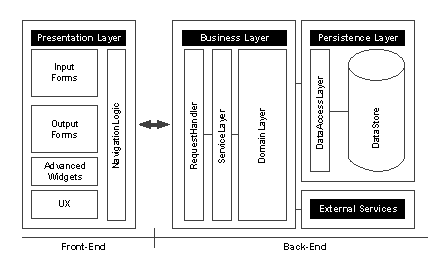
\includegraphics[width=\linewidth,keepaspectratio=true]{images/enterpriseLayers/enterpriseLayers.eps}
	\end{center}
\end{frame}

\begin{frame}[c]
	\frametitle{Responsabilidades de la Capa de Presentación}
	\begin{enumerate}[<+->]
        \item Permitir a los usuarios interactuar con el sistema.
        \item Introducir datos en el sistema (validándolos previamente).
        \item Visualizar los datos de salida de manera amigable al usuario.
        \item Facilitar operaciones simples (filtros, ordenaciones y cambios de formato) sobre los datos.
        \item Facilitar la navegación por el sistema.
        \item Mejorar la experiencia de usuario (UX). %% Hellmans
        \item Gestionar la comunicación con el servidor.
        \item Gestionar situaciones excepcionales.
	\end{enumerate}
\end{frame}

\begin{frame}[c]
	\frametitle{Responsabilidades de la Capa de Negocio}
	\begin{enumerate}[<+->]
        \item Atender las peticiones de los clientes.
        \item Asegurar el cumplimiento de \alert{reglas de negocio} existentes.
        \item Asegurar la \alert{transaccionalidad} de las operaciones de negocio.
        \item Validar las peticiones de los clientes.
        \item Recuperar y almacenar datos del almacén o almacenes persistentes.
        \item Facilitar la eficiencia del sistema.
        \item Controlar el acceso a los datos.
        \item Gestionar la comunicación con los servicios externos.
        \item Ejecutar operaciones (periódicas) del sistema.
        \item Gestionar de manera adecuada casos excepcionales.
        \item Ayudar a satisfacer los requisitos no funcionales.
	\end{enumerate}
\end{frame}

\begin{frame}[c]
	\frametitle{Responsabilidades de la Capa de Persistencia}
	\begin{enumerate}[<+->]
        \item Almacenar los datos de manera no volátil.
        \item Recuperar datos del almacén persistente.
        \item Asegurar la disponibilidad de los datos.
        \item Controlar la integridad de los datos.
        \item Asegurar un acceso eficiente a los datos.
	\end{enumerate}
\end{frame}

\subsection[SIEs Web]{Sistemas de Información Empresariales Web}

\begin{frame}[c]
    \frametitle{Sistema Informático Web}
    %% TODO: Buscar una definición mejor o más estandarizada.
    \begin{block}{Sistema Informático Web}
        Un \emph{Sistema Informático Web} es un sistema cliente servidor donde el cliente está codificado utilizando tecnologías web, como HTML, CSS y Javascript, siendo por tanto accesible desde un navegador web; y/o donde el cliente se comunica con el servidor por medio del protocolo HTTP.
    \end{block}
\end{frame}

\begin{frame}[c]
	\frametitle{¿Por Qué se Utilizan Tecnologías Web?}
    \centering \textbf{Ventajas} \\
    \begin{enumerate}
        \item<2-> Multiplataforma.
        \item<3-> Onmipresencia de la web.
        \item<4-> No precisan permisos especiales a nivel de red.
        \item<5-> Facilidad de mantenimiento (código móvil).
        \item<6-> Fuerte estandarización.
        \item<7-> Favorecen la \emph{recognizability}, reduciendo su curva de aprendizaje.
        \item<8-> Madurez de las herramientas.
    \end{enumerate}
    \uncover<9->{
        \centering \textbf{Inconvenientes} \\
        \begin{enumerate}
            \item<10-> Seguridad.
            %% https://goo.gl/ypz4VD
            \item<11-> Tecnologías originalmente desarrolladas para \emph{hipertexto}.
            \item<12-> Tecnologías lentas.
            \item<13-> Tecnologías dependientes de terceros.
        \end{enumerate}
    }
\end{frame}

\subsection[Tecnologías SIE]{Tecnologías de Implementación para Arquitecturas Empresariales}

\begin{frame}[c]
	\frametitle{Tecnologías de Implementación SIEs}
	\begin{center}
        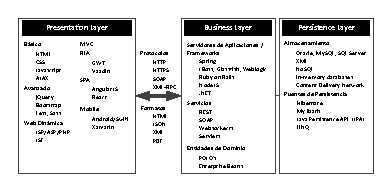
\includegraphics[width=\linewidth,keepaspectratio=true]{images/enterpriseLayers/technologies.eps}
	\end{center}
\end{frame}

\subsection{Distribución de Capas en Arquitecturas Empresariales}

\begin{frame}[c]
	\frametitle{Despliegue de Aplicaciones Empresariales}
	\begin{enumerate}[<+->]
        \item Front-end en el cliente y back-end en uno o más servidores.
        \item Dominio y persistencia pueden ir en el mismo servidor (\emph{two tier}) o en servidores separados (three tiers).
        \item Los clientes pueden ser pesados (PCs) o ligeros (Smartphones, tablets).
        \item Trabajo sin conexión puede requerir parte de la capa de dominio (y persistencia) en el cliente.
        \item La capa de presentación puede ser de código fijo (app, desktop) o móvil (HTML + Javascript).
	\end{enumerate}
\end{frame}

\section{Inversión e Inyección de Dependencias}

\subsection{Principio de Inversión de Dependencias}

\begin{frame}[c]
	\frametitle{Principio de Inversión de Dependencias}
    \begin{block}{Principio de Inversión de Dependencias (IoD)}
        Las clases de un sistema software deberían depender de abstracciones estables y no de implementaciones concretas.
    \end{block}
\end{frame}

\begin{frame}[c]
	\frametitle{Problema a Resolver I}
	\begin{center}
        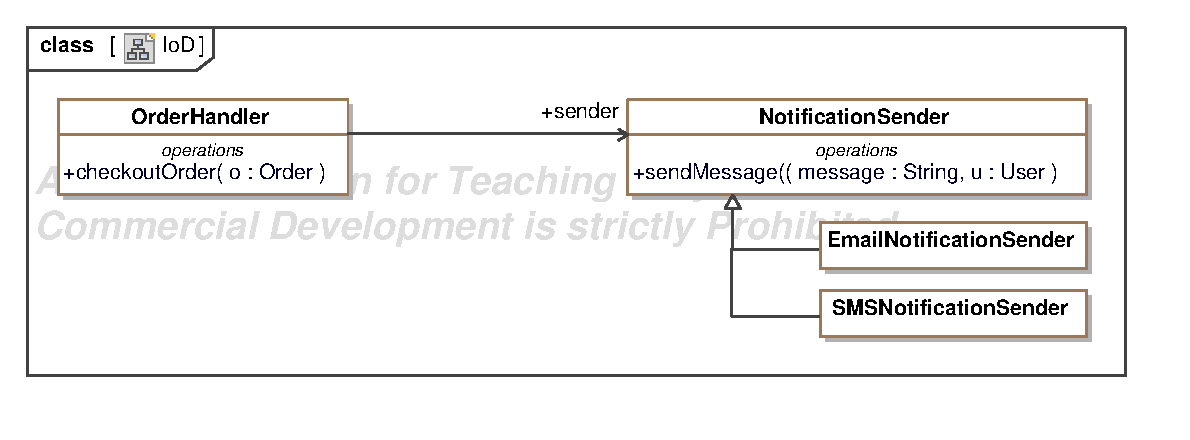
\includegraphics[width=\linewidth,keepaspectratio=true]{images/IoD/IoD.eps}
	\end{center}
\end{frame}

\begin{frame}[c,fragile]
	\frametitle{Problema a Resolver II}
\begin{lstlisting}[basicstyle=\footnotesize,language=Java]
public class OrderHandler {

  // Depende de la clase abstracta
  protected NotificationSender sender;

  public OrderHandler() {
    //Al instanciarlo queda ligado a una clase concreta.
    this.sender = new SmsNotificationSender();
  } // Constructor
  ...
}
\end{lstlisting}
\end{frame}

\subsection{Inversión por Constructor}

\begin{frame}[c,fragile]
	\frametitle{Inversión de Dependencias por Constructor}
\begin{lstlisting}[basicstyle=\footnotesize,language=Java]
public class OrderHandler {

  protected NotificationSender sender;
	
  public OrderHandler(NotificationSender aSender) {
	this.sender =  aSender;
  } // Constructor
  ...
}
\end{lstlisting}
\end{frame}

\begin{frame}[c,fragile]
	\frametitle{Inversión de Dependencias por Constructor}
\begin{lstlisting}[basicstyle=\footnotesize,language=Java]
public static void main(String[] args) {
  NotificationSender ns = new SmsNotificationSender();
  OrderHandler oh = new OrderHandler(ns);
}
\end{lstlisting}
\end{frame}

\subsection{Inversión por Setter}

\begin{frame}[c,fragile]
	\frametitle{Inversión de Dependencias por \emph{Setter}}
\begin{lstlisting}[basicstyle=\footnotesize,language=Java]
public class OrderHandler {

  protected NotificationSender sender;
	
  public OrderHandler() {}
	
  public void setSender(NotificationSender aSender) {
    this.sender = aSender;
  }
  ...
}
\end{lstlisting}
\end{frame}

\subsection{Inyección de Dependencias}

\begin{frame}[c]
	\frametitle{Problema a Resolver}
	\begin{center}
        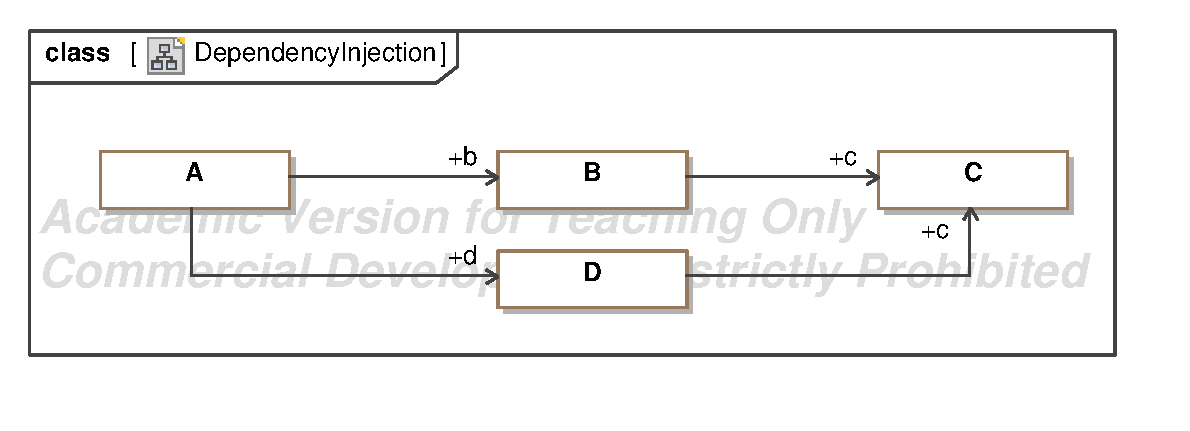
\includegraphics[width=\linewidth,keepaspectratio=true]{images/iod/DependencyInjection.eps}
	\end{center}
\end{frame}

\begin{frame}[c,fragile]
	\frametitle{Problema a Resolver}
\begin{lstlisting}[basicstyle=\footnotesize,language=Java]
public static void main(String[] args) {
  // Para crear A me hace falta ...
  C c1 = new C_X();
  D d1 = new D_X(c1);
  C c2 = new C_X();
  B b1 = new B_X(c2);
  A a  = new A_X(b1,d1);
}
\end{lstlisting}
\end{frame}

\begin{frame}[c]
	\frametitle{Solución - Inyector de Dependencias}
    \begin{itemize}[<+->]
        \item En un fichero de configuración, se especifican las subclases concretas a usar por cada clase abstracta.
        \item Se marcan de algún modo las dependencias a inyectar.
        \item Se crean objetos \alert{sin parámetros} a través de una facilidad externa denominada \emph{inyector de dependencias}.
        \item El inyector se encarga de crear los parámetros necesarios instanciando las subclases adecuadas conforme al fichero de configuración.
    \end{itemize}
\end{frame}

\subsection{Inyección de Dependencias en Spring}

\subsubsection{Inyección Simple}

\begin{frame}[c,fragile]
	\frametitle{Inyección Simple - Definición}
\begin{lstlisting}[basicstyle=\footnotesize,language=Java]
@Component
public class OrderHandler {

  @Autowired
  protected NotificationSender sender;
	
  public OrderHandler() {}
	
  public void processOrder(Order o) {
    this.sender.sendMessage("Order accepted",o.getUser());
  }
}
\end{lstlisting}
\end{frame}

\begin{frame}[c,fragile]
	\frametitle{Inyección Simple - Creación}
\begin{lstlisting}[basicstyle=\footnotesize,language=Java]
public class Runner {

  @Autowired
  protected ApplicationContext context;

  @Override
  public void run(String... arg0) throws Exception {
    	
    oh = context.getBean(OrderHandler.class);
    ...
    oh.processOrder(o);
  }
}\end{lstlisting}
\end{frame}

\subsubsection{Inyección Basada en Cualificadores}

\begin{frame}[c,fragile]
	\frametitle{Inyección Basada en Cualificadores I}
\begin{lstlisting}[basicstyle=\footnotesize,language=Java]
@Component
@Qualifier("EmailNotifications")
public class EmailNotificationSender extends NotificationSender {

  @Override
  public void sendMessage(String message, User u) {}
	
}
\end{lstlisting}
\end{frame}

\begin{frame}[c,fragile]
	\frametitle{Inyección Basada en Cualificadores II}
\begin{lstlisting}[basicstyle=\footnotesize,language=Java]
@Component
public class OrderHandler {

  @Autowired
  @Qualifier("EmailNotifications")
  protected NotificationSender sender;
	
  public OrderHandler() {}
	
  public void processOrder(Order o) {
    this.sender.sendMessage("Order accepted",o.getUser());
  }
}
\end{lstlisting}
\end{frame}

\subsubsection{Inyección Basada en Anotaciones de Configuración}

\begin{frame}[c,fragile]
	\frametitle{Inyección Basada en Anotaciones de Configuración I}
\begin{lstlisting}[basicstyle=\footnotesize,language=Java]
@Component
public class OrderHandler {

  @Autowired
  protected NotificationSender sender;
	
  public OrderHandler() {}
	
  public void processOrder(Order o) {
    this.sender.sendMessage("Order accepted",o.getUser());
  }
}
\end{lstlisting}
\end{frame}

\begin{frame}[c,fragile]
	\frametitle{Inyección Basada en Anotaciones de Configuración II}
\begin{lstlisting}[basicstyle=\footnotesize,language=Java]
@Configuration
public class IoD_DemoConfig {
	
  @Bean
  public NotificationSender sender() {
    return new SmsNotificationSender();
  }
}
\end{lstlisting}
\end{frame}

\subsubsection{Inyección Basada en Configuración XML}

\begin{frame}[c,fragile]
	\frametitle{Inyección Basada en Configuración XML I}
\begin{lstlisting}[basicstyle=\footnotesize,language=XML]
<?xml version="1.0" encoding="UTF-8"?>
<beans
   xmlns="http://www.springframework.org/schema/beans"
   ...>
   <bean class="[...].iod.OrderHandler" autowire="byName">
   </bean>
   <bean id="sender"
         class="[...].iod.EmailNotificationSender">
   </bean>
</beans>
\end{lstlisting}
\end{frame}

\begin{frame}[c,fragile]
	\frametitle{Inyección Basada en Configuración XML II}
\begin{lstlisting}[basicstyle=\footnotesize,language=Java]
@SpringBootApplication
@ImportResource("classpath:ApplicationContext.xml")
public class Runner implements CommandLineRunner {
\end{lstlisting}
\end{frame}

\section{Sumario y Referencias}

\begin{frame}[c]
    \frametitle{¿Qué Tengo que Saber de Todo Esto?}
    \begin{enumerate}[<+->]
        \item Comprender el concepto de \emph{Sistema de Información Empresarial}.
        \item Comprender el concepto de \emph{Arquitectura Sw}.
        \item Conocer los principios, ventajas e inconvenientes de las arquitecturas en capas, cliente-servidor y de código móvil.
        \item Comprender qué es un sistema sw web, sus ventajas e inconvenientes.
        \item Comprender por qué se divide un SIE en capas.
        \item Conocer algunas de las tecnologías para la implementación de un SIE.
        \item Comprender cómo se distribuyen las capas de un SIE.
        \item Comprender qué es la \emph{inversión de dependencias}.
        \item Comprender qué es la \emph{inyección de dependencias}.
        \item Ser capaz de invertir dependencias \emph{por constructor} y \emph{por setter}.
        \item Conocer cómo se inyectan dependencias en Spring.
    \end{enumerate}
\end{frame}

\begin{frame}
	\frametitle{Referencias}
    \nocite{}
	\bibliographystyle{apalike}
    \bibliography{ae-tema1}
\end{frame}

\end{document} 